\newthought{With Pending inquiry,} we have the ability to cancel multiple orders at the same time.

This can be useful in cases where all the orders on a container need to be canceled (I.e. a CBC and ADIFF are clotted.)


\paragraph{Select} the orders which need to be canceled.\sidenote{To select multiple orders hold down the Ctrl key while clicking additional orders.}\\

\prettyimage{width=.8\textwidth, trim={2pt, 30pt, 15pt, 3pt}, clip}{graphics/pending_inquiry}

\paragraph{Click} the \btn{graphics/cancel_icon} \textsc{Cancel Icon} from the \textsc{Tool bar}.\sidenote{\trouble{If part of the order has been resulted, Cerner will display a message saying: ``The selected Order Cannot be Canceled ''

The rest of the order must be resulted with a \textsc{Freetext} result and the test must be credited.}}\\

\prettyimage{width=\textwidth}{graphics/toolbar}

\paragraph{Review} the information to ensure the right order has been selected.\sidenote{Check that the Order(s) and Patient's name are correct.}\\

\prettyimage{width=.4\textwidth}{graphics/cancel_order_start}

\paragraph{Select} the appropriate Cancel Reason from the drop-down menu.\sidenote{In this case we will choose: ``Specimen Clotted. To be recollected.''}\\

\prettyimage{width=.45\linewidth, trim={0, 50pt, 0, 0}, clip}{graphics/cancel_reasons}


\paragraph{Click}the  \btn{graphics/comment_icon.png} icon to open the \textsc{Cancel Comment window}.\sidenote{The \textsc{Cancel Comment Window} will open. }

\newthought{Enter any required } comments:\begin{marginfigure}
          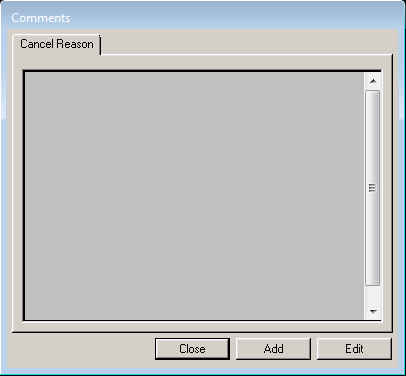
\includegraphics[width=0.8\linewidth]{graphics/cancel_comment_dialog.png}
\end{marginfigure}

\begin{description}
    % \begin{itemize}
      \paraitem{Click} the \btn{graphics/edit_button.png} button.
      \paraitem{Enter} any required comments.
      \paraitem{Click} \btn{graphics/ok_button.png}  when finished.
      \paraitem{Click} \btn{graphics/close_button.png} to close the Comments dialog.
    % \end{itemize}
\end{description}\marginnote{For more information on entering comments: \checkref{part:comments}{\refpt{part:comments}}{Refer to the \boldcap{Comments} documentation}.}

\paragraph{Review} the information, ensuring everything is correct.\\

\prettyimage{width=.5\textwidth}{graphics/cancel_order_done}

\paragraph{Click} \btn{graphics/cancel_order_button.png}  when finished.

\newthought{Pending Inquiry will} refresh, and the canceled tests will no long be visible.
